\documentclass{article}
%compile this file with: xelatex proposal.tex

\usepackage[utf8]{inputenc}
\usepackage{graphicx}
\usepackage{lipsum}
\usepackage{url}
\usepackage{hyperref}
\usepackage{indentfirst}
\usepackage{xeCJK}
\setCJKmainfont{SimSun}
\hypersetup{
    colorlinks=true,
    linkcolor=blue,
    filecolor=magenta,
    urlcolor=cyan,
}

% Title
\title{Examining the Efficacy of LLMs in Comprehending Homophones}
\author{Clair Ross\\Nuoqi Liu}
\date{\today}

\begin{document}

\maketitle

\section{Introduction}

Homophones are words that sounds similar but have different meanings, like 'new' and 'knew'. This phenomenon is rare in English, but extremely frequent in certain languages, like Chinese. Homophones can be manually created easily for almost every Chinese word. As an example, the word 警察 (policeman) sounds exactly the same as 井茶 (tea in the well), 景查 (scenery and investigation) and 颈猹 (neck and badger).

Manually created homophones are commonly used for pranks, and for bypassing censorship in social media. Human can understand such homophone expressions easily. However, it is suprising that state-of-the-art LLMs like ChatGPT has no ability at all in understanding such homophone expressions. In this study, we will build a test set, and use it to measure some state-of-the-art LLMs' ability in comprehending homophone expressions.

\section{Objectives}

A test set of 100 questions about Chinese homophones will be created manually. One example question goes as:

\begin{figure}[h]
    \centering
    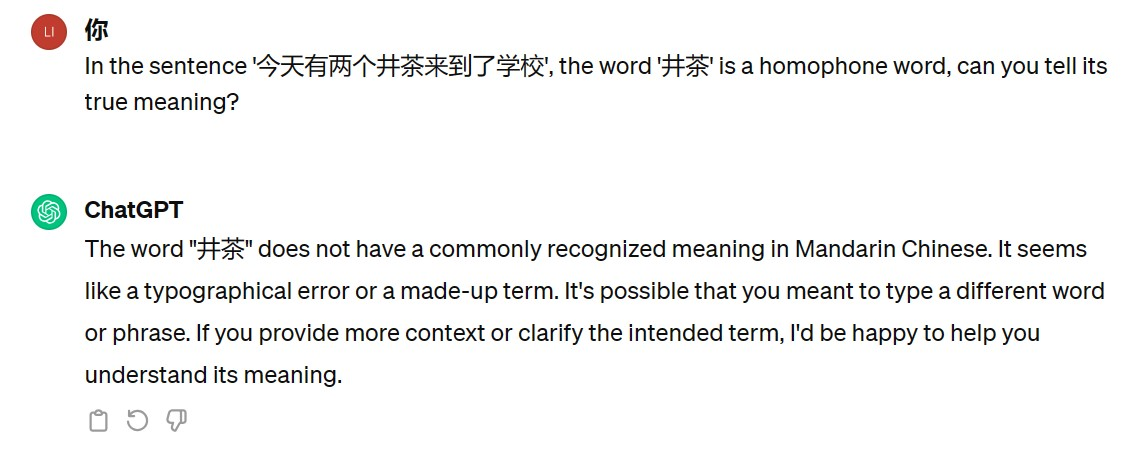
\includegraphics[width=0.9\textwidth]{example_question_chinese.jpg}
\end{figure}

Also, a similar test set of 100 questions about Spanish homophones will also be created. One example question goes as:

\begin{figure}[h]
    \centering
    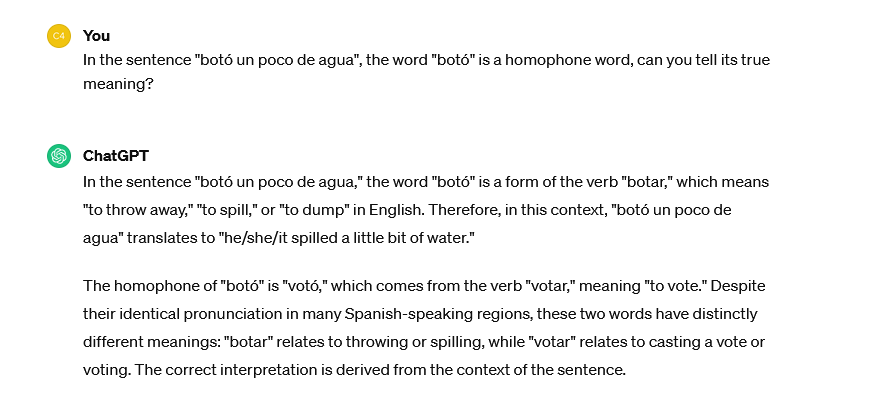
\includegraphics[width=0.9\textwidth]{example_question_spanish.png}
\end{figure}

The test set will be ran on 5 LLMs or translators. The performance for each model will be measured and analyzed. Possible strategies to improve the performance, like chain-of-thought prompting, will be tried and analyzed.

\section{Evaluation Metrics}

LLM's efficacy of comprehending homophones will be measures by accuracy on test set. For the example question '今天有两个井茶来到了学校', if the correct answer '警察' or 'policeman' is shown in LLM's reply, the answer is marked as correct.

\section{Task Division}

Firstly, all group members will read the related papers, to get a broader view of this topic.

Nuoqi Liu will create the Chinese homophone test set, run the test set on 5 LLMs.

Ross Clair will create the Spanish homophone test set, run the test set on 5 LLMs.

Nuoqi Liu will undertake the task of data analysis and academic writing.

Ross Clair will undertake the task of literature review.

\section{Existing Literature}

We found no study focusing on this topic. Most study focus on homophones in voice chat other than text chat. Some papers partly related to this topic includs:

\href{https://arxiv.org/abs/2401.07441}{Stability Analysis of ChatGPT-based Sentiment Analysis in AI Quality Assurance}

\href{https://arxiv.org/abs/2312.13585}{Speech Translation with Large Language Models: An Industrial Practice}

We plan to read these papers, and hopefully get some enlightenment.

\end{document}
